% !TeX document-id = {fb8a2ef5-cdaf-49da-b79d-0a8152e677cd}
% !TeX TS-program = XeLaTeX
\documentclass[a4paper,12pt]{report}

% polyglossia should go first!
\usepackage{polyglossia} % multi-language support
\setmainlanguage{russian}
\setotherlanguage{english}

\usepackage{amsmath} % math symbols, new environments and stuff
\usepackage{unicode-math} % for changing math font and unicode symbols
\usepackage[style=english]{csquotes} % fancy quoting
\usepackage{microtype} % for better font rendering
\usepackage{hyperref} % for refs and URLs
\usepackage{graphicx} % for images (and title page)
\usepackage{geometry} % for margins in title page
\usepackage{tabu} % for tabulars (and title page)
\usepackage[section]{placeins} % for float barriers
\usepackage{titlesec} % for section break hooks
\usepackage{listings} % for listings 
\usepackage{upquote} % for good-looking quotes in source code (used for custom languages)
\usepackage{xcolor} % colors!
\usepackage{enumitem} % for unboxed description labels (long ones)
\usepackage{caption}

\defaultfontfeatures{Mapping=tex-text} % for converting "--" and "---"
\setmainfont{CMU Serif}
\setsansfont{CMU Sans Serif}
\setmonofont{CMU Typewriter Text}
\setmathfont{XITS Math}
\MakeOuterQuote{"} % enable auto-quotation

% new page and barrier after section, also phantom section after clearpage for
% hyperref to get right page.
% clearpage also outputs all active floats:
\newcommand{\sectionbreak}{\phantomsection}
\newcommand{\subsectionbreak}{\FloatBarrier}
\renewcommand{\thesection}{\arabic{section}} % no chapters
\numberwithin{equation}{section}
%\usetikzlibrary{shapes,arrows,trees}

\newcommand{\itemtt}[1][]{\item[\texttt{#1}:]} % tt-ed items (for protocol descriptions)

\definecolor{bluekeywords}{rgb}{0.13,0.13,1}
\definecolor{greencomments}{rgb}{0,0.5,0}
\definecolor{turqusnumbers}{rgb}{0.17,0.57,0.69}
\definecolor{redstrings}{rgb}{0.5,0,0}
\setmonofont{Consolas} %to be used with XeLaTeX or LuaLaTeX
\definecolor{bluekeywords}{rgb}{0,0,1}
\definecolor{greencomments}{rgb}{0,0.5,0}
\definecolor{redstrings}{rgb}{0.64,0.08,0.08}
\definecolor{xmlcomments}{rgb}{0.5,0.5,0.5}
\definecolor{types}{rgb}{0.17,0.57,0.68}

\lstset{language=[Sharp]C,
captionpos=b,
%numbers=left, %Nummerierung
%numberstyle=\tiny, % kleine Zeilennummern
frame=lines, % Oberhalb und unterhalb des Listings ist eine Linie
showspaces=false,
showtabs=false,
breaklines=true,
showstringspaces=false,
breakatwhitespace=true,
escapeinside={(*@}{@*)},
commentstyle=\color{greencomments},
morekeywords={partial, var, value, get, set},
keywordstyle=\color{bluekeywords},
stringstyle=\color{redstrings},
basicstyle=\ttfamily\small,
}

\lstset{
  numbers=left,
  numberstyle=\scriptsize,
  basicstyle=\ttfamily\scriptsize,
  columns=fullflexible,
  keepspaces, % for spaces in unicode text!
  captionpos=b
}
\renewcommand{\lstlistingname}{Листинг}

\date{\today}

\makeatletter
\let\thetitle\@title
\let\theauthor\@author
\let\thedate\@date
\makeatother

\makeatletter
\AtBeginDocument{%
    \expandafter\renewcommand\expandafter\subsection\expandafter{%
        \expandafter\@fb@secFB\subsection
    }%
}
\makeatother

\begin{document}

\clearpage
\section*{Введение}

\clearpage
\section{Аналитическая часть}

\subsection{Проектирование общей структуры комплекса}
В ходе разработки была составлена схема комплекса. Схема приведена на рис.~\ref{fig:schema}. Функционал каждой компоненты описан в таблице~\ref{tab:schema}.

\begin{figure}[h!]
    \centering
    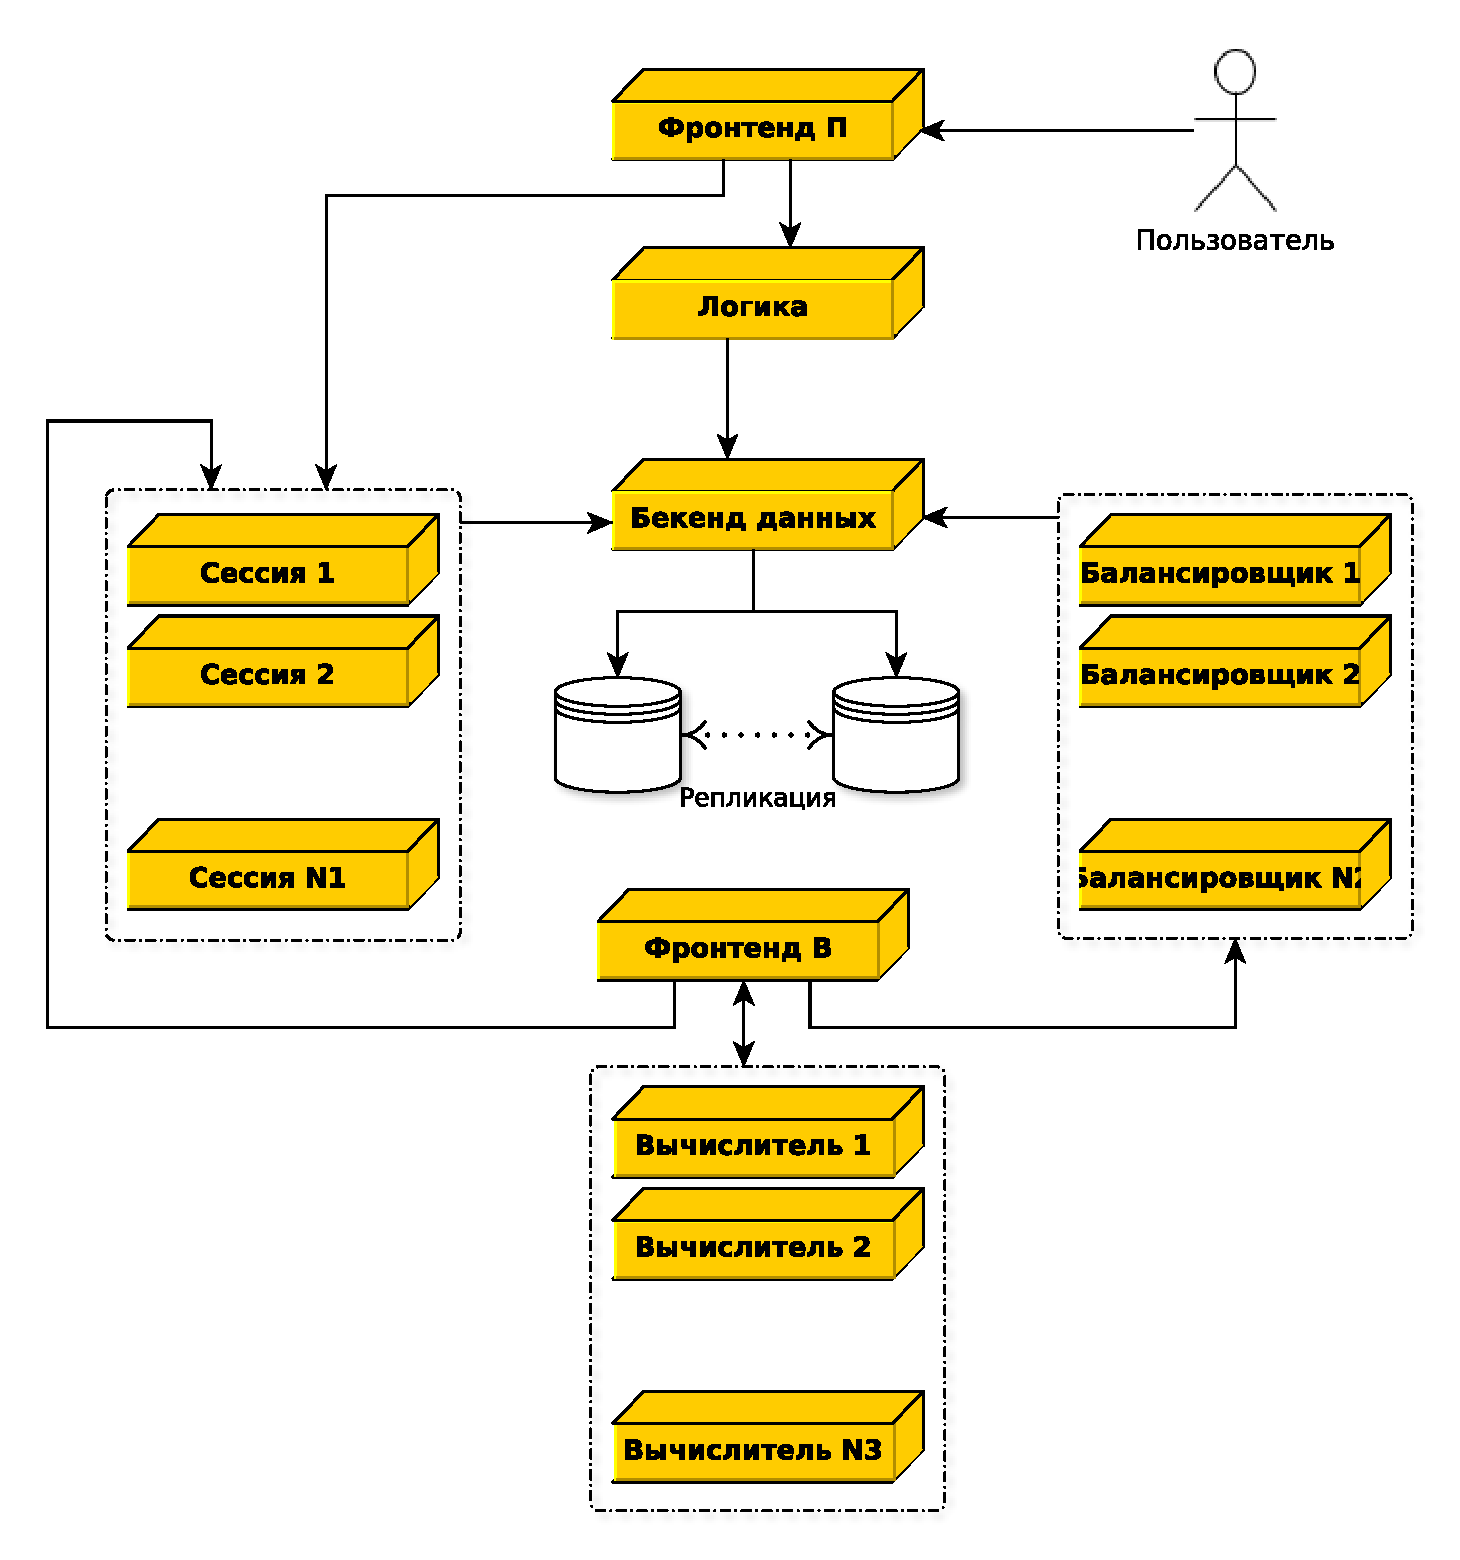
\includegraphics[width=.6\linewidth]{img/schema}
    \caption{Схема комплекса}
    \label{fig:schema}
\end{figure}

\begin{table}[h!]
  \caption{Описание элементов схемы на рис.~\ref{fig:schema}}
  \label{tab:schema}
  \begin{tabu}{|c|X[c]|}
    \hline
    Название сервиса   & Функционал сервиса                                                                            \\ \hline
    Логика             & Реализация пользовательского интерфейса в виде API либо веб-страницы                          \\ \hline
    Бекенд данных      & Инкапсуляция доступа к БД                                                                     \\ \hline
    Сессия 1..N        & Аутентификация и авторизация пользователей                                                    \\ \hline
     Балансировщик 1..N & Отслеживание состояния вычислителей, выдача им новых задач, сбор результатов выполнения задач \\ \hline
      Фронтенд П,В       & Проверка прав пользователей на доступ к предоставляемому API                                  \\ \hline
  \end{tabu}
\end{table}

\subsection{Проектирование базы данных}
\subsubsection{Определение требований к структуре БД}
БД должна осуществлять функцию коммуникации между отдельными узлами сети.
Это накладывает следующие требования на её структуру:
\begin{itemize}
  \item Чтобы по возможности уменьшить степень дублирования похожих описаний задач, в отдельную сущность должны быть вынесены "черты" задач (traits). Чертой, к примеру, является требование задачи к вычислителю иметь окружение "Cuda v4.0" или ".net 3.5".
  \item Чтобы позволить отслеживать состояние всех подзадач задачи, запущенной с дублированием вычислений, в отдельную сущность должны быть вынесены "подзадачи", наследующие все атрибуты родительской задачи и хранящие данные, относящиеся непосредственно к ходу вычислений (на каком вычислителе производятся вычисления, результат вычислений и т д).
  \item Чтобы комплекс имел возможность выбора подходящего вычислительного узла для задачи, вычислительным узлам (Agents) должны соответствовать такие же наборы "черт", как и диспетчеризуемой в данный момент задаче.
\end{itemize}

\subsubsection{ER-диаграмма}
С учётом вышеописанных ограничений на структуру, отношения сущностей в базе данных можно представить в виде ER-диаграммы на рис.~\ref{fig:db-erd}.

\begin{figure}
    \centering
    \includegraphics[width=\linewidth]{img/db-er-crowsfoot}
    \caption{ER-диаграмма сущностей в базе данных}
    \label{fig:db-erd}
\end{figure}

\subsubsection{Таблица полей и типов данных}
Атрибуты отдельных сущностей в базе данных хранятся в полях типов, описанных в таблице~\ref{tab:db-types}. Каждой сущности соответствует отдельная таблица. Запись вида "T?" в столбце "Тип" означает, что значение необязательно. Обязательные поля-идентификаторы не указаны в таблице.

\begin{table}
  \caption{Типы полей таблиц}
  \label{tab:db-types}
  \begin{tabu}{|c|c|X[c]|X[c]|}
    \hline
        Таблица     &     Поле      & Тип                               & Описание                    \\ \hline
        Subtask     &   AgentUsed   & UID?                              & Использованный узел         \\ \cline{2-4}
                    &    Status     & \shortstack{Scheduled, In process \\ Terminated, N/A \\ Completed}    & Статус задачи \\ \cline{2-4}
                    &  ResultFile   & string?                           & Имя архива с результатами   \\ \hline
         Task       &  ConfigFile   & string                            & Имя конфигурационного файла \\ \hline
         Agent      &      --       & --                                & --                          \\ \hline
         Trait      &     Name      & string                            & Имя черты                   \\ \cline{2-4}
                    &   Version     &    string                         & Версия черты                \\ \hline
  \end{tabu}
\end{table}

\subsection{Проектирование API отдельных сервисов}
\subsubsection{Сервер БД}
REST API, полное отражение структуры БД на набор эндпойнтов-объектов (/agents/id, /traits/id, tasks/id и т д)

\subsubsection{Балансировщик}
\begin{tabu}{|c|c|X[c]|}
  \hline
          Функционал          &    Endpoint     & Хедеры-параметры                 \\ \hline
    Получение новой задачи    &  GET /newtask   & AgentID                          \\ \hline
  Выдача результатов расчёта  &  POST /result   & AgentID, SubtaskID, Status, Body \\ \hline
  Оповещение о статусе работы & POST /heartbeat & AgentID                          \\ \hline
\end{tabu}

\subsubsection{Фронтенд вычлительных узлов}
Дублирует эндпойнты балансировщика; добавлены функции:
\begin{itemize}
  \item Регистрация нового узла в сети
  \item Подключение зарегистрированного узла к сети
\end{itemize}
Запросы на эндпойнты балансировщика проходят проверку безопасности и уходят к балансировщику(ам), запросы на регистрацию/подключение идут сразу к серверу сессии.

\subsubsection{Сервер сессии}
Отвечает за аутентификацию пользователей на обоих фронтендах. 
В случае несоответствия ключей безопасности ожидаемым запрос не пропускается "внутрь" комплекса.
Внутри комплекса - "доверенная" область, проверок безопасности нет.

\subsubsection{Сервер логики}
Должен обеспечивать функционал:
\begin{itemize}
  \item Регистрация нового пользователя
  \item Вход пользователя в свой аккаунт
  \item Постановка новой задачи на выполнение
  \item Просмотр статусов поставленных задач
  \item Для выполненых задач - получение результатов в виде архива
\end{itemize}

\subsubsection{Пользовательский фронтенд}
Дублирует эндпойнты сервера логики, проверяя ключи перед перенаправлением запроса на сервер логики.

\end{document}